\subsection{ROLLO: Reactor evOLutionary aLgorithm Optimizer}
\begin{frame}
    \frametitle{ROLLO: Reactor evOLutionary aLgorithm Optimizer}
    \begin{figure}
        
\includegraphics[width=0.7\linewidth]{figures/rollo-logo.png} 
        \caption{ROLLO (Reactor evOLutionary aLgorithm Optimizer) logo.}
    \end{figure}
    \begin{itemize}
        \item ROLLO (Reactor evOLutionary aLgorithm Optimizer) is a Python package 
        that applies evolutionary algorithms to optimize nuclear reactor design
        \item ROLLO provides a general genetic algorithm framework, sets up 
        parallelization for the user, and promotes usability with an input file that
        only exposes mandatory parameters
        \item Design Goals: effective, flexible, open-source, parallel,
        reproducible
    \end{itemize}
\end{frame}

\begin{frame}
    \frametitle{ROLLO: Reactor evOLutionary aLgorithm Optimizer}
    \begin{minipage}[c]{0.45\textwidth}
        \begin{itemize}
            \item ROLLO initially reads and validates the JSON input file, initializes 
            the DEAP genetic algorithm hyperparameters and operators, and finally runs
            the genetic algorithm following the flow chart, in which the nuclear 
            software evaluates each individual reactor model's fitness.
        \end{itemize}
        \end{minipage}\hfill
        \begin{minipage}[c]{0.52\textwidth}
            \centering
            \begin{figure}
                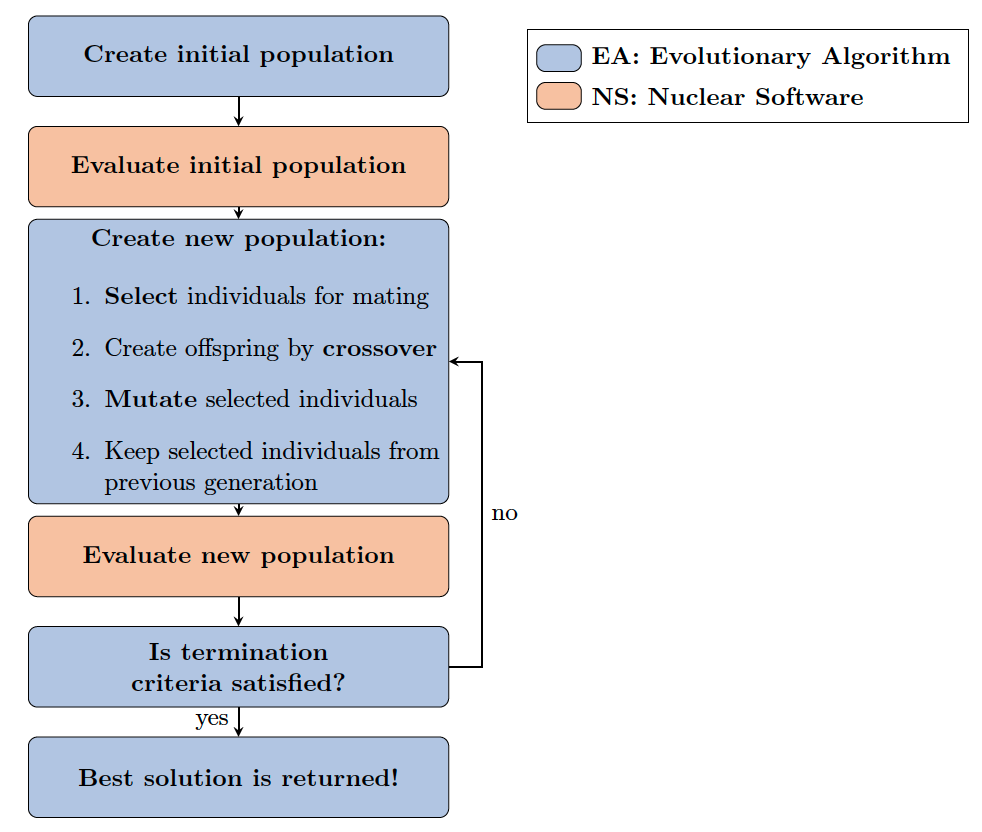
\includegraphics[width=\linewidth]{figures/rollo-flow.png} 
                \caption{Optimization tool's flow.}
            \end{figure}
        \end{minipage}
\end{frame}

\subsection{ROLLO Verification}
% verification? 
\subsection{Optimization Methodology}
% methodology for optimization... 
\subsection{AHTR Plank Optimization Results}
\subsection{AHTR One-Third Assembly Optimization Results}